% !TeX root = ../main.tex
\chapter{Balance de potencia del enlace}
\label{cap:enlace}

\section{Introducci\'on}
\label{sec:enl-intro}

Los cap\'itulos anteriores desarrollaron por separado los tres bloques
fundamentales del enlace LEO--GEO. El modelo del canal y su principal fuente de
ruido (\cref{cap:canal}), el modelo del transmisor y el receptor \'opticos
(\cref{cap:transceptor}) y el procesamiento digital que compensa las
imperfecciones de los dos anteriores (\cref{cap:dsp}). Este cap\'itulo los
re\'une para analizar la viabilidad del enlace en t\'erminos de potencia.

Se realiza un balance de potencia donde se identifican las ganancias y las
p\'erdidas de cada etapa, y se establece una relaci\'on entre la potencia del
l\'aser transmisor y la OSNR a la entrada del receptor. Con los resultados de
simulaci\'on de la cadena completa se cuantifican las penalidades respecto del
l\'imite te\'orico de un receptor ideal en un canal AWGN, y se determina el
umbral de operaci\'on del sistema.

El cap\'itulo cierra con las simplificaciones del balance y con los t\'erminos
que quedaron fuera por el alcance del proyecto.
\section{Balance de potencia}
\label{sec:enl-linkbudget}

En el \cref{ap:ruido} se desarrolla el an\'alisis te\'orico que determina la
OSNR m\'inima necesaria para alcanzar el umbral de BER del esquema de
correcci\'on de errores. Para el sistema DP-QPSK de este trabajo ese requisito
es de \SI{12.61}{\dB}, suponiendo un receptor ideal sobre un canal AWGN. A
partir de ah\'i, el balance de potencia recorre las ganancias y las p\'erdidas
de cada etapa para determinar qu\'e potencia \'optica tiene que entregar el
l\'aser transmisor.

\paragraph{Relaci\'on entre potencia de l\'aser y OSNR:}
Sea $\Pcw$ la potencia \'optica emitida por el l\'aser transmisor, medida a la
entrada del modulador. El modulador DP introduce p\'erdidas por la conversi\'on
intr\'inseca de los MZM, por el acoplamiento a fibra y por la propagaci\'on a
trav\'es de las gu\'ias de onda y el rotador de polarizaci\'on. Para los
c\'alculos que siguen se tom\'o como referencia el modulador de niobato de
litio del laboratorio, que a \SI{32}{\giga\baud} especifica una p\'erdida de
inserci\'on total de hasta
\begin{equation}
  L_{\mathrm{DP}} = \SI{14}{\dB}
  \label{eq:liqm}
\end{equation}
seg\'un su hoja de datos~\cite{fujitsu_ftm7977}.

Considerando la ganancia del amplificador \'optico de transmisi\'on,
$G_b = \SI{35}{\dB}$, y la p\'erdida neta del enlace de la
\eqref{eq:pathloss}, la potencia \'optica a la entrada del pre-amplificador del
receptor resulta
\begin{equation}
  P_{rx} = \Pcw - L_{\mathrm{DP}} + G_b - L = \Pcw - \SI{52.40}{\dB}.
  \label{eq:prx}
\end{equation}

A la salida del pre-amplificador la potencia de se\~nal es
$P_{rx} + G_{\mathrm{EDFA}}$. La potencia total de ruido ASE que la acompa\~na
en el ancho de referencia es
$P_{\mathrm{ASE}} = 10\log_{10}\!\left(2S_{\mathrm{pol}}\Bref/\SI{1}{\milli\watt}\right)
= \SI{-28.46}{\dBm}$, con $S_{\mathrm{pol}}$ la densidad espectral de potencia
de ruido por cada uno de los dos modos de polarizaci\'on, definida en la
\eqref{eq:ase}. El cociente entre ambas potencias es la OSNR de la
\eqref{eq:osnr-def},
\begin{equation}
  \OSNR\,[\si{\dB}]
    = \underbrace{\left(P_{rx} + G_{\mathrm{EDFA}}\right)}_{\text{se\~nal en }\si{\dBm}}
      - \underbrace{P_{\mathrm{ASE}}}_{\text{ASE en }\si{\dBm}}
    = \Pcw\,[\si{\dBm}] - 52{,}40 + 25{,}0 + 28{,}46,
  \label{eq:osnr-pcw-pasos}
\end{equation}
que se reduce a una \'unica constante aditiva,
\begin{equation}
  \OSNR\,[\si{\dB}] = \Pcw\,[\si{\dBm}] + 1{,}06.
  \label{eq:osnr-pcw}
\end{equation}
Los dos t\'erminos que se restan en la \eqref{eq:osnr-pcw-pasos} est\'an en
\si{\dBm}, de modo que su diferencia es un cociente y queda en \si{\dB}. La
constante de la \eqref{eq:osnr-pcw} va sin unidad porque arrastra esa
cancelaci\'on de la referencia de \SI{1}{\milli\watt}.

Esta expresi\'on vincula el balance con las simulaciones del
\cref{cap:tolerancias}. Fijar una OSNR objetivo equivale a fijar la potencia
\'optica que tiene que entregar el l\'aser transmisor.

\begin{figure}[H]
  \centering
  \begin{tikzpicture}[font=\footnotesize, >={Latex[length=2mm]}, yscale=0.115, xscale=1.02]
    \definecolor{cSig}{RGB}{11,90,127}
    \definecolor{cAse}{RGB}{194,51,41}

    % --- ejes -----------------------------------------------------------
    \foreach \y in {-40,-30,-20,-10,0,10,20,30}{
      \draw[gray!25] (-0.35,\y) -- (11.7,\y);
      \node[left, gray!55!black, font=\scriptsize] at (-0.40,\y) {\y};
    }
    \draw[->, gray!60!black] (-0.35,-45) -- (-0.35,37);
    \node[rotate=90, gray!55!black, font=\scriptsize, above] at (-1.15,-4)
         {potencia \'optica [dBm]};

    % --- escalones de senal ---------------------------------------------
    \draw[cSig, very thick]
       (0.00,12.54) -- (1.60,12.54)
    -- (1.60,-1.46) -- (3.90,-1.46)
    -- (3.90,33.54) -- (6.20,33.54)
    -- (6.20,-39.86) -- (8.50,-39.86)
    -- (8.50,-14.86) -- (10.90,-14.86);

    % --- nivel de ASE ----------------------------------------------------
    \draw[cAse, thick, dashed] (8.50,-28.46) -- (11.10,-28.46);
    \node[cAse, right, font=\scriptsize, align=left] at (11.05,-28.46)
         {ASE total\\ en $\Bref$\\ \SI{-28.5}{\dBm}};

    % --- flecha de OSNR --------------------------------------------------
    \draw[<->, thick, black] (9.60,-14.86) -- (9.60,-28.46);
    \node[right, font=\scriptsize, align=left] at (9.70,-21.7)
         {\textbf{OSNR}\\ \SI{13.6}{\dB}};

    % --- etiquetas de cada tramo ----------------------------------------
    \node[cSig, above, font=\scriptsize] at (0.80,12.54)  {\SI{12.5}{\dBm}};
    \node[cSig, below, font=\scriptsize] at (2.75,-1.46)  {\SI{-1.5}{\dBm}};
    \node[cSig, above, font=\scriptsize] at (5.05,33.54)  {\SI{33.5}{\dBm} = \SI{2.3}{\watt}};
    \node[cSig, below, font=\scriptsize] at (7.35,-39.86) {\SI{-40.0}{\dBm}};
    \node[cSig, above, font=\scriptsize] at (10.35,-14.86) {\SI{-15.0}{\dBm}};

    % --- etiquetas de los saltos ----------------------------------------
    \node[right, font=\scriptsize, align=left] at (1.70,5.5)
         {modulador DP\\ $-\SI{14}{\dB}$};
    \node[right, font=\scriptsize, align=left] at (4.00,17.0)
         {booster\\ $+\SI{35}{\dB}$};
    \node[right, font=\scriptsize, align=left] at (6.30,-6.0)
         {enlace\\ $-\SI{73.4}{\dB}$};
    \node[right, font=\scriptsize, align=left] at (8.60,-35.5)
         {preamp.\\ $+\SI{25}{\dB}$};

    % --- eje de etapas ---------------------------------------------------
    \node[below, font=\scriptsize, gray!55!black] at (0.80,-46)  {l\'aser};
    \node[below, font=\scriptsize, gray!55!black] at (2.75,-46)  {mod.};
    \node[below, font=\scriptsize, gray!55!black] at (5.05,-46)  {booster};
    \node[below, font=\scriptsize, gray!55!black] at (7.35,-46)  {espacio};
    \node[below, font=\scriptsize, gray!55!black] at (9.70,-46)  {preamp.};
  \end{tikzpicture}
  \caption[Balance de potencia del enlace]{%
    Nivel de potencia \'optica a lo largo de la cadena, evaluado en el punto de
    operaci\'on de vuelo, es decir en el umbral HD-FEC y a la distancia del
    peor instante del pase. La l\'inea de trazos es el ASE total del
    pre-amplificador medido en el ancho de referencia. La separaci\'on entre
    ambas al final de la cadena es la OSNR.}
  \label{fig:balance}
\end{figure}

La \cref{fig:balance} muestra la evoluci\'on de la potencia \'optica a lo largo
del enlace, y la \cref{tab:balance} presenta el balance desglosado por etapas.

\begin{table}[htbp]
  \centering

  \begin{tabular}{lrr}
    \toprule
    T\'ermino & Modulador real & Modelo de modulador \\
    \midrule
    Potencia del l\'aser CW, $\Pcw$   & \SI{12.5}{\dBm}  & \SI{4.7}{\dBm} \\
    P\'erdida del modulador DP        & \SI{-14.0}{\dB}  & \SI{-6.2}{\dB} \\
    Ganancia del booster              & \SI{+35.0}{\dB}  & \SI{+35.0}{\dB} \\
    \midrule
    \textbf{Potencia transmitida}         & \SI{33.5}{\dBm}  & \SI{33.5}{\dBm} \\
    \midrule
    P\'erdida neta del enlace         & \SI{-73.4}{\dB}  & \SI{-73.4}{\dB} \\
    \midrule
    \textbf{Entrada del pre-amplificador} & \SI{-40.0}{\dBm} & \SI{-40.0}{\dBm} \\
    \midrule
    Ganancia del pre-amplificador     & \SI{+25.0}{\dB}  & \SI{+25.0}{\dB} \\
    Potencia de se\~nal               & \SI{-15.0}{\dBm} & \SI{-15.0}{\dBm} \\
    ASE total en $\Bref$              & \SI{-28.5}{\dBm} & \SI{-28.5}{\dBm} \\
    \midrule
    \textbf{OSNR}                     & \SI{13.6}{\dB}   & \SI{13.6}{\dB} \\
    \bottomrule
  \end{tabular}
  \caption[Balance de potencia]{%
    Balance de potencia t\'ermino por t\'ermino, evaluado en el umbral
    operativo y a $d = \SI{45000}{\kilo\metre}$, el peor instante del pase. Las
    dos columnas describen el mismo enlace y difieren en un \'unico t\'ermino,
    el modelo de p\'erdida del modulador.}
  \label{tab:balance}
\end{table}

Las dos columnas de la \cref{tab:balance} consideran modelos distintos de
p\'erdida del modulador. El modelo de la \cref{sec:trx-modulador} contempla
\'unicamente la p\'erdida de conversi\'on intr\'inseca de los MZM, estimada en
\SI{6.2}{\dB} a excursi\'on plena. El balance de dise\~no, en cambio, usa la
p\'erdida de inserci\'on total del dispositivo real, los \SI{14}{\dB} de la
\eqref{eq:liqm}. Esa diferencia de \SI{7.8}{\dB} se compensa con un incremento
equivalente en la potencia del l\'aser, de manera que ambos modelos dan la
misma potencia \'optica a la salida del modulador y, en consecuencia, los
mismos niveles de potencia y de OSNR en el resto del enlace. La relaci\'on que
reporta la \eqref{eq:osnr-pcw} es la del modulador real.

\paragraph{Validez del modelo lineal:}
La \eqref{eq:osnr-pcw} supone ganancias y p\'erdidas constantes a lo largo del
enlace. Los amplificadores \'opticos, sin embargo, saturan, y su ganancia
depende de la potencia de entrada. La aproximaci\'on vale mientras los dos
amplificadores de la cadena trabajen en r\'egimen lineal.

El pre-amplificador no presenta problemas. Por la \eqref{eq:prx}, en el punto
de operaci\'on su entrada es de \SI{-40.0}{\dBm}, muy por debajo de cualquier
nivel de compresi\'on, de modo que su ganancia de \SI{25}{\dB} puede tomarse
constante. La figura de ruido de \SI{4.5}{\dB} que adopta el modelo del
\cref{ap:ruido} es consistente con los valores reportados para
pre-amplificadores de fibra validados por radiaci\'on para enlaces l\'aser
satelitales~\cite{edmunds2017}.

El booster es el que define el dimensionamiento, porque opera con una potencia
de salida pr\'oxima a su l\'imite de saturaci\'on. En el punto de operaci\'on
esa potencia es
\begin{equation}
  P_{\mathrm{out}} = \Pcw - L_{\mathrm{DP}} + G_b = \SI{33.5}{\dBm}
                   \equiv \SI{2.3}{\watt}.
  \label{eq:pout-booster}
\end{equation}

Considerando un m\'odulo de \SI{5}{\watt} de potencia nominal de salida y
\SI{40}{\dB} de ganancia m\'axima~\cite{nuphoton}, equivalente a una potencia
de saturaci\'on $P_{\mathrm{sat}} = \SI{37.0}{\dBm}$, el amplificador trabaja
\begin{equation}
  P_{\mathrm{sat}} - P_{\mathrm{out}} = \SI{3.5}{\dB}
  \label{eq:backoff}
\end{equation}
por debajo de la saturaci\'on. Su entrada de \SI{-1.5}{\dBm} tambi\'en cae
dentro del rango de operaci\'on especificado para este tipo de m\'odulos.

\paragraph{Umbral operativo y m\'argenes de potencia:}
Con la penalidad de implementaci\'on y los deterioros de vuelo que se obtienen
en la \cref{sec:enl-verificacion}, la OSNR m\'inima para operar por debajo del
umbral HD-FEC queda en \SI{13.6}{\dB}. Por la \eqref{eq:osnr-pcw} eso
corresponde a $\Pcw = \SI{12.5}{\dBm}$, unos \SI{18}{\milli\watt}. El l\'aser
comercial disponible en el laboratorio entrega hasta \SI{17}{\dBm} en banda
C~\cite{ppcl500}, de modo que quedan \SI{4.5}{\dB} de margen respecto de su
m\'axima potencia de emisi\'on.

La potencia m\'axima que puede alcanzar la se\~nal en el receptor, sin embargo,
no la limita el l\'aser sino la saturaci\'on del booster,
\begin{equation}
  \OSNR_{\max} = P_{\mathrm{sat}} - L + G_{\mathrm{EDFA}} - P_{\mathrm{ASE}}
               = \SI{17.0}{\dB}.
  \label{eq:osnr-max}
\end{equation}
Ese valor representa un margen de \SI{3.5}{\dB} sobre la OSNR m\'inima
requerida, evaluado a la m\'axima distancia del enlace. La principal
limitaci\'on de potencia del sistema queda entonces del lado del booster, y no
del l\'aser transmisor. El margen se podr\'ia ampliar con un amplificador de
transmisi\'on de mayor potencia de saturaci\'on.

\section{Penalidad de implementaci\'on y umbral operativo}
\label{sec:enl-verificacion}

Para evaluar el desempe\~no del sistema y determinar la OSNR m\'inima de
operaci\'on se simul\'o la cadena completa, con el modelo del transceptor del
\cref{cap:transceptor} y el DSP del \cref{cap:dsp}. El resultado se compara con
la curva te\'orica de BER de un receptor ideal sobre un canal AWGN, la
\eqref{eq:ber-qpsk}.

Se corren dos configuraciones. La primera es el receptor sin los deterioros de
vuelo, y sirve para cuantificar la penalidad que introducen las limitaciones
del receptor y el error residual de los algoritmos del DSP. La segunda
representa la condici\'on m\'as exigente del enlace, con el desplazamiento
Doppler, el error de frecuencia de reloj, el desajuste de fase de muestreo, el
ancho de l\'inea y el RIN de los l\'aseres, la deriva del estado de
polarizaci\'on, el skew y el error de cuadratura actuando de manera
simult\'anea. Los valores son los de especificaci\'on del enlace y se detallan
en la \cref{tab:tol-configs}.

\begin{figure}[H]
  \centering
  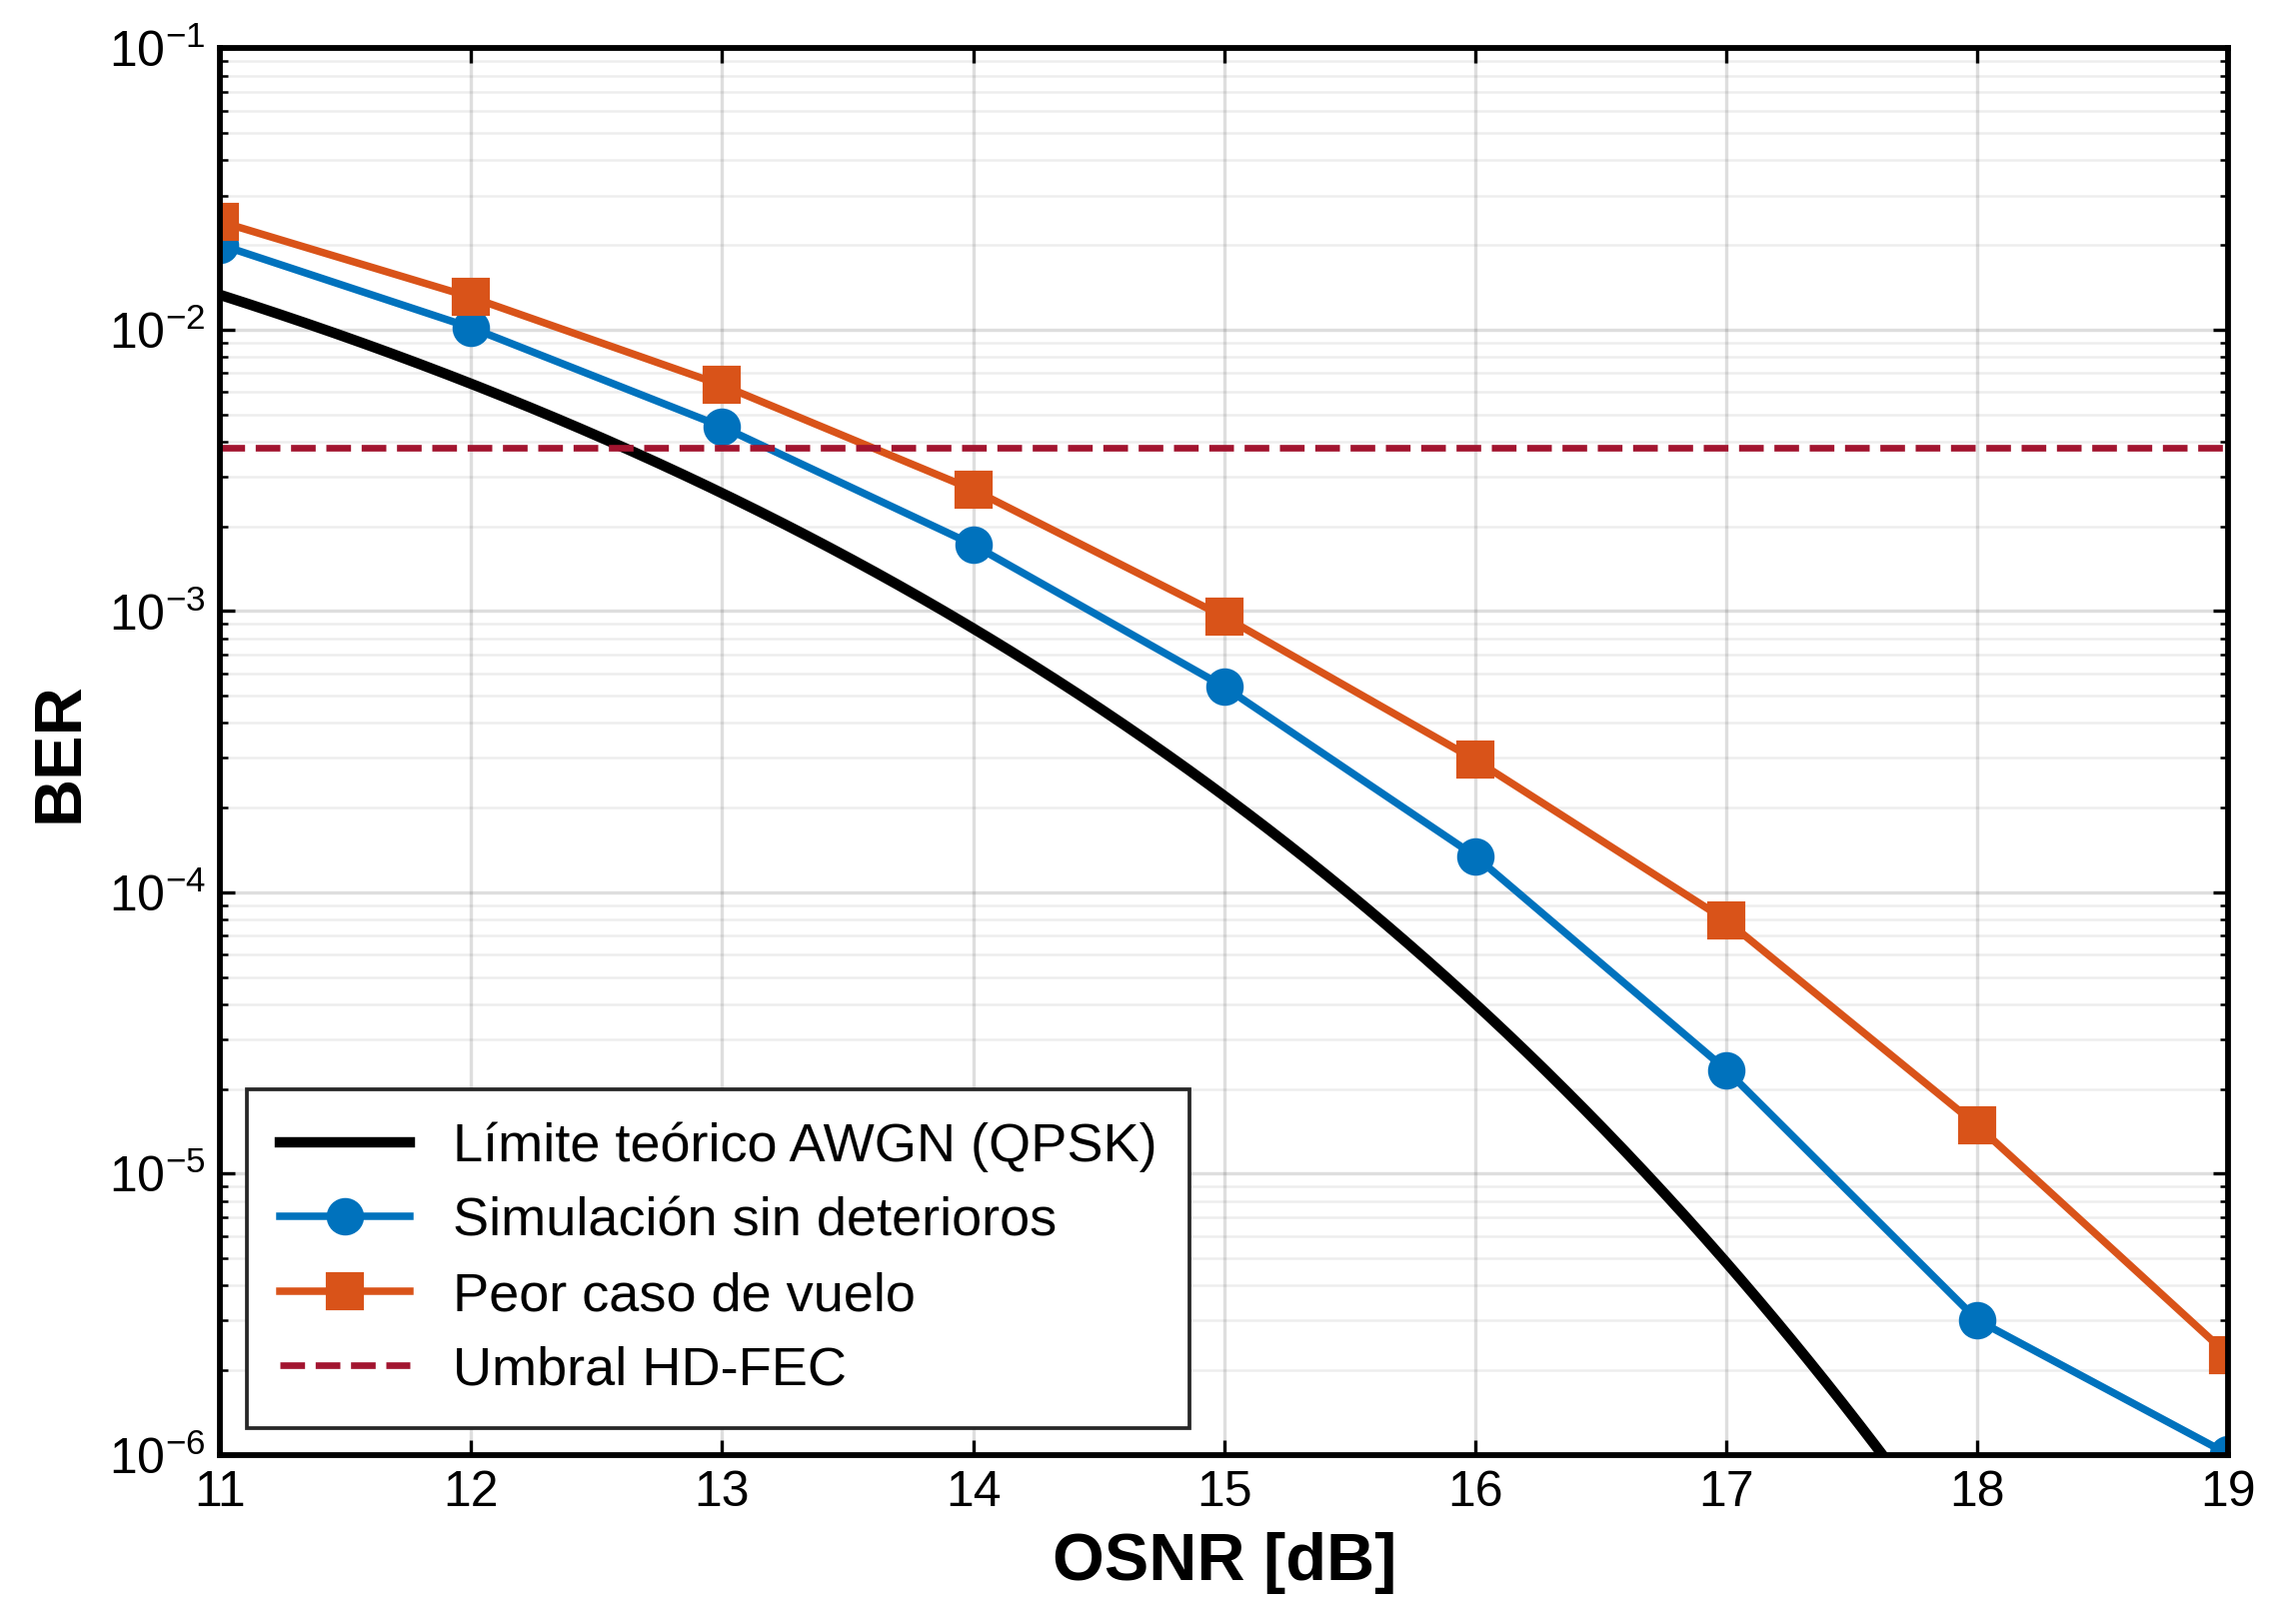
\includegraphics[width=0.85\textwidth]{figuras/ber_vs_osnr.png}
  \caption[Desempe\~no simulado contra el l\'imite te\'orico]{%
    BER contra OSNR. La curva negra es el l\'imite te\'orico AWGN de la
    \cref{eq:ber-qpsk}. La curva azul representa la cadena completa sin
    desbalances y la naranja, el peor caso de vuelo. Las dos separaciones
    horizontales sobre el umbral HD-FEC son la penalidad de implementaci\'on
    del receptor y el costo de los deterioros de vuelo.}
  \label{fig:ber-osnr}
\end{figure}

Como se observa en la \cref{fig:ber-osnr}, en ausencia de deterioros el umbral
HD-FEC se alcanza con una $\OSNR$ de \SI{13.18}{\dB}, frente a los
\SI{12.61}{\dB} del receptor ideal de la \cref{tab:cadena-teorica}. Esa
diferencia representa una penalidad de implementaci\'on de \SI{0.57}{\dB},
atribuible a las limitaciones del receptor y al error residual de los
algoritmos de compensaci\'on del DSP. Al incorporar los deterioros de vuelo de
manera simult\'anea, la OSNR requerida sube a \SI{13.60}{\dB}, es decir
\SI{0.42}{\dB} m\'as. La \cref{tab:umbral} resume los resultados.

\begin{table}[htbp]
  \centering

  \begin{tabular}{llc}
    \toprule
    Configuraci\'on & Penalidad & $\OSNR$ en el umbral \\
    \midrule
    Te\'orico AWGN            & ---                                   & \SI{12.61}{\dB} \\
    Receptor sin deterioros   & $+\SI{0.57}{\dB}$ de implementaci\'on & \SI{13.18}{\dB} \\
    Peor caso de vuelo        & $+\SI{0.42}{\dB}$ de deterioros       & \SI{13.60}{\dB} \\
    \bottomrule
  \end{tabular}
  \caption[Descomposici\'on del umbral operativo]{%
    Penalidad desde el receptor ideal al umbral operativo. La \'ultima fila es
    la que se usa en el balance de potencia.}
  \label{tab:umbral}
\end{table}

De los dos t\'erminos, el mayor es la penalidad de implementaci\'on. Los
deterioros de vuelo con valores de especificaci\'on aportan menos de medio
decibel entre todos.
\section{T\'erminos no contemplados en el balance}
\label{sec:enl-critica}

Se enumeran ciertos aspectos del balance que no se tienen en cuenta, o se simplifican por el alcance del proyecto:
\begin{puntos}
\item{La p\'erdida de apuntamiento es una estimaci\'on:}
En un enlace real el apuntamiento no es un error fijo sino un proceso aleatorio, y es controlado por el Sistema de Control de Actitud (ACS). Sin embargo, para simplicidad se utiliz\'o \SI{5}{\dB} 
de p\'erdidas constantes por este fen\'omeno.

\item{Falta el acoplamiento a fibra monomodo:}
El balance lleva la potencia desde el telescopio de recepci\'on hasta la
entrada del pre-amplificador sin ning\'un t\'ermino intermedio. En realidad, el
haz recibido tiene que acoplarse a una fibra monomodo. En este proceso se tienen dos tipos 
de p\'erdidas. En primer lugar est\'a el desajuste entre el campo de una apertura circular
uniformemente iluminada y el modo gaussiano de la fibra. Por otro lado, se tiene el error de frente de onda residual del
telescopio. Ninguno de estos efectos se tuvo en cuenta debido a la complejidad de sus implementaciones.


\item{No hay margen de sistema asignado:}
El balance se cierra con \SI{3.5}{\dB} entre el umbral operativo y el
l\'imite de saturaci\'on del booster, sin reservar margen para la degradaci\'on
de los componentes a lo largo de la vida \'util. Esto incluye el envejecimiento del l\'aser, la
deriva t\'ermica del punto de polarizaci\'on del modulador y las tolerancias
de fabricaci\'on entre unidades, que una misi\'on real cubre con un margen de
sistema reservado desde el dise\~no.

\end{puntos}
El resultado es que el balance de potencia cierra o no seg\'un las penalidades de estos factores. Un an\'alisis detallado de los subsistemas del sat\'elite es una continuaci\'on natural del proyecto.
\section{Conclusiones}
\label{sec:enl-conclusiones}

El balance de potencia permiti\'o evaluar la viabilidad del enlace LEO--GEO
bajo las condiciones de dise\~no consideradas. A \SI{45000}{\kilo\metre}, los
componentes de la \cref{tab:balance} alcanzan la OSNR necesaria para operar por
debajo del umbral HD-FEC, con un margen de \SI{3.5}{\dB} hasta la saturaci\'on
del booster.

La simulaci\'on completa cuantific\'o una penalidad de implementaci\'on de
\SI{0.57}{\dB} respecto del l\'imite te\'orico AWGN, a la que se suman
\SI{0.42}{\dB} asociados a los deterioros de vuelo. El requisito de OSNR para
el dimensionamiento del enlace queda entonces en \SI{13.60}{\dB}.

El balance no contempla las p\'erdidas de acoplamiento a fibra monomodo ni
reserva un margen de sistema para degradaciones e incertidumbres adicionales.
Las p\'erdidas por apuntamiento, adem\'as, se aproximaron con una penalidad
constante de \SI{5}{\dB}. La viabilidad del enlace queda condicionada a que
estos efectos se mantengan dentro del margen disponible. Por \'ultimo, el
an\'alisis se hizo cerca de la separaci\'on m\'axima entre los sat\'elites, de
modo que operar a distancias menores deja m\'as margen de potencia.
